%-----------------------------------------------------------------------------%
%                                                                             %
%    K A P I T E L   2                                                        %
%                                                                             %
%-----------------------------------------------------------------------------%

\chapter{Background: Optimal Bipedal Locomotion}\label{c2}
The second chapter provides the reader with fundamentals on the mathematical modeling of legged robots, outlines how motion generation can be formulated as optimization problem and introduces the class of algorithms used within this thesis. 

%\section{Modeling and Control of Legged Robots}
\section{Foundations of Bipedal Locomotion}
\subsection{Terminology}
In order to describe the locomotion of a humanoid robot, some specific terms are required that are introduced within this section. \citeauthor{vukobratovic2007towards} provide an extensive introduction to the terminology related to bipedal walking, concisely summarized by \citeauthor{dekker2009zero} \cite{vukobratovic2007towards, dekker2009zero}.\\\\
\textbf{Walk}\\
Walk can be defined as: "\textit{Movement by putting forward each foot in turn, not having both feet off the ground at once}".\\\\
\textbf{Run}\\
Run in turn is characterized by  a movement where partially both feet leaving the ground at the same time.\\\\
\textbf{Gait}\\
The way each human walks and runs is unique, hence gait can be defined as: "\textit{Manner of walking or running}".\\\\
\textbf{Periodic gait}\\
If a gait is realized by repeating each locomotion phase in an identical way, the gait is referred to as \textit{periodic}.\\\\
\textbf{Symmetric gait}\\
If the left and right leg move in an identical but time-shifted manner, the gait is referred to as \textit{symmetric}.\\\\
\textbf{Double Support}\\
A situation where the humanoid has two isolated contact surfaces with the ground.\\\\
\textbf{Single Support}\\
A situation where  the humanoid has only one contact surface with the ground.\\\\
\textbf{Support Polygon}\\%TODO: Maybe add figure to illustrate single vs double support
The support polygon is formed by the \textit{convex hull} about the ground contact points.    \\\\
\textbf{Swing foot}\\
This term refers to the leg that is performing a step, i.e. moving through the air.\\\\
\textbf{Supporting foot}\\
This term refers to the leg that is in contact with the ground, supporting all the weight of the humanoid. 

\subsection{Dynamic Modeling of Legged Robots}
In this section we will introduce the equations of motion for a manipulator as well as for  floating base systems. A concise introduction to this topic is presented with \cite{scaronTeaching}, more comprehensive studies can be found in \cite{roboticSystemsLab2017, featherstone2014rigid}.
\subsubsection{General Formulation}
Mathematical models of a robot's dynamics describe the motion as a function of time and control inputs. These models are the basis for both simulation and control of robotic systems. In an abstract form, the \gls{EoM} are written as: 
\begin{equation} \label{eqn:EoMGeneral}
F(\bq(t),\bdq(t),\bddq(t),\bu(t),t)=0,
\end{equation}
where 
\begin{itemize}
\item \myM{t} is the time variable, 
\item \myM{q} is the vector of generalized coordinates,
\item $\bdq$ is the first time derivative (velocity) of \myM{q}, 
\item $\bddq$ is the second time derivative (acceleration) of \myM{q} and
\item \myM{u} is the vector of control inputs. 
\end{itemize}
Consequently, the \gls{EoM} provide a mapping between the control space on the one hand and the state space of robot on the other hand. Typical methods for computing the closed-form solution of the \gls{EoM} are e.g. the classical \textit{Newton-Euler} method or the \textit{Lagrange method}, where the former is based on principles for conservation of linear and angular momenta and the latter utilizes energy-based functions expressed in generalized coordinates. 
\subsubsection{Manipulator Equations}
For applications with fixed-based robots, e.g. a robotic manipulator, the multi-body dynamics can be formulated as
\begin{equation} \label{eqn:EoMManipulator}
\myM{M}(\bq)\bddq+\bdq^T\myM{C}(\bq)\bdq=\btau+\btau_g(\bq),
\end{equation}
where 
\begin{itemize}
\item $\myM{M}(\bq)$ is the generalized inertia matrix, 
\item $\myM{C}(\bq)$ is the coriolis tensor, 
\item $\btau$ is the vector of actuated joint torques and 
\item $\btau_g(\bq)$ is the vector of external joint torques caused by gravity.
\end{itemize}
In contrast to the general formulation \cref{eqn:EoMGeneral}, this expression is time-invariant. Hence, \cref{eqn:EoMManipulator} can be used to calculate the acceleration $\bddq$ based on the given state $(\bq, \bdq)$, also known as \gls{FD}, as well as the \gls{ID}.
\subsubsection{Floating Base Systems (Legged Robots)}
A floating base system is characterized by having a base that is free to move, rather than being fixed in space. Consequently, the vector of generalized coordinates $\bq$ not only contains the joints angles, but also accounts for the position and orientation of the floating base. Legged robots belong to this category of rigid-body systems as they make and brake contacts with their environment in order to move. Contrary to manipulators, contacts need to be actively enforced by kinematic contact constraints for legged robots. There are namely two different types of contact constraints that can be applied: point contacts (3d) or surface contacts (6d). 
For the case of point contacts, the dynamics of the floating base system become
\begin{equation*} \label{eqn:EoMLeggedRobotPtContact}
\myM{M}(\bq)\bddq+\bdq^T\myM{C}(\bq)\bdq=\myM{S}^T\btau+\btau_g(\bq)+\sum_{i=1}^{k}\myM{J}_{C_i}^T\myM{f}_i,
\end{equation*}
where 
\begin{itemize}
\item \myM{S} is the selection matrix of actuated joints,
\item $\myM{J}_{C_i}$ is the Jacobian at the location of a contact point $C_i$ and
\item $\bfun_i$ is the contact force acting at the contact point $C_i$.
\end{itemize}
For the case of surface contacts, such as a flat foot on the floor, modeling a point contact is not sufficient since it only constrains the translation. In order to also account for the rotational constraints enforced by the geometry one could take into account multiple point contacts. A non-redundant alternative is to model more general frame contact constraints as
\begin{equation*} \label{eqn:EoMLeggedRobotSurfaceContact}
\myM{M}(\bq)\bddq+\bdq^T\myM{C}(\bq)\bdq=\myM{S}^T\btau+\btau_g(\bq)+\sum_{i=1}^{k}\myM{J}_{C_i}^T\myM{w}_i,
\end{equation*}
where $\myM{w}_i$ is referred to as the \textit{contact wrench} acting on the contact link $i$. This wrench stacks the resultant $\bfun_i$ of contact forces and the moment $\myM{m}_i$ exerted by these forces around the contact frame as
$$\myM{w}_i=\{\myM{f}_i,\myM{m}_i\}.$$ 
For more details on contact wrenches and spatial vector algebra in general, the interested reader is referred to e.g. \cite[Ch.2]{featherstone2014rigid}.

%\subsection{Motion Generation}
%\subsection{Motion Control}
%\subsubsection{Kinematic Control (High-gain joint position trajectory tracking)}
%\subsubsection{Impedance Control with Joint Space Inverse Dynamics (Low-gain joint control with model compensation)}
%\subsubsection{Task Space Inverse Dynamics Control (Directly regulating in «task space»)}
%\subsubsection{Virtual Model Control (Dynamic control of a quasistatic system)}
%\subsection{Efficient Walking}


\section{Contact Stability Analysis}
Overview of stability margins in \cite{garcia2002classification} and for Handbook of Robotics see main reference from tedrake \cite{pratt2006velocity}; 
CoM and CoP calculation and coincidence described in \cite{sardain2004forces}.

\subsection{Stability Criteria}

\subsubsection{Floor Projection of the Center of Mass (FCoM)}
\begin{equation*} 
\bp_{CoM}=\dfrac{\sum_{i=1}^{n}m_i\bp_i}{\sum_{i=1}^{n}m_i}
\end{equation*}
\begin{equation*} 
\sum_{i=1}^{n}((\bp_{FCoM}-\bp_i)\times m_i\myM{g})=\myM{0}
\end{equation*}
\subsubsection{Zero-Moment Point (ZMP)}
Introduction in \cite{vukobratovic1972stability}, reviewed in \cite{vukobratovic2004zero}, made popular with \cite{kajita2003biped}.
Assumptions:
\begin{itemize}
\item One planar contact are (i.e. no multiple surfaces like on rough terrain)
\item Sufficiently high friction to prevent sliding of the feet
\end{itemize}
%TODO
% Describe CoP and ZMP according to https://scaron.info/teaching/zero-tilting-moment-point.html
\subsubsection{Center of Pressure (CoP)}
Conditions for \gls{CoP} inside convex hull:
\begin{align}
\begin{split}
\mid\mid\tau^x\mid\mid &\leq Yf^z \\
\mid\mid\tau^y\mid\mid &\leq Xf^z 
\end{split}
\end{align}
Which can be modeled by the four inequality conditions:
\begin{align}
\begin{split}
\tau^x &\leq Yf^z \\
-\tau^x &\leq Yf^z \\
\tau^y &\leq Yf^z \\
-\tau^y &\leq Yf^z 
\end{split}
\end{align}
These conditions are be implemented via: 
\begin{equation}
\begin{bmatrix} 0 & 0 & -Y & 1 & 0 & 0 \\
0 & 0 & -Y & -1 & 0 & 0 \\
0 & 0 & -X & 0 & 1 & 0 \\
0 & 0 & -X & 0 & -1 & 0 \end{bmatrix} \cdot
\begin{bmatrix} f^x \\ f^y \\ f^z \\ \tau^x \\ \tau^y \\ \tau^z \end{bmatrix} \leq
\begin{bmatrix} 0 \\ 0 \\ 0 \\ 0 \end{bmatrix}
\end{equation}

\subsubsection{Backup: Friction Cone constraints}
\begin{align}
\begin{split}
\mid\mid f^x\mid\mid &\leq \mu f^z \\
\mid\mid f^y\mid\mid &\leq \mu f^z \\
f^z &> 0
\end{split}
\end{align}
For the case of four edges of the linear approximation of the friction cone, the equations become:
\begin{equation}
\begin{bmatrix} 1 & 0 & -\mu \\
-1 & 0 & -\mu \\
0 & 1 & -\mu \\
0 & -1 & -\mu \\
0 & 0 & -\mu \\ \end{bmatrix} \cdot
\begin{bmatrix} f^x \\ f^y \\ f^z \end{bmatrix} \leq
\begin{bmatrix} 0 \\ 0 \\ 0 \\ 0 \\ 0 \end{bmatrix}
\end{equation}

\subsubsection{Coincidence of ZMP and CoP}

\subsection{Stability Classification}
There are existing several classifications on stability, which will be defined in the following according to \cite[Sec.1.2.1]{westervelt2018feedback} and \cite{garcia2002classification}. See \citeauthor{vukobratovic2007towards} for more details on differentiating the terms dynamic stability and dynamic balance \cite{vukobratovic2007towards}.  

\subsubsection{Statically Stable Gait}
The gait or movement of a humanoid is classified as \textit{statically stable}, if the \gls{FCoM} does not leave the \gls{SP} during the entire motion or gait. Consequently, the humanoid will remain in a stable position, whenever the movement is stopped. Typically, these kind of stability are only obtained with very low walking velocities or quasi-static motions, where the static forces dominate the dynamic forces.  

\subsubsection{Dynamically Stable Gait}
If the \gls{FCoM} partially leaves the \gls{SP} at some point during the gait, but the \gls{CoP} (or \gls{ZMP}) always remains within the \gls{SP}, the gait or movement is classified as \textit{dynamically stable}. This stability margin is extremely useful for flat-foot dynamic walking since it prevents the foot from rotating around the boundary of the \gls{SP}. 


\section{Differential Dynamic Programming (DDP)}\label{sec:DDP}
This section describes the basics of \gls{DDP}, which is an \gls{OC} algorithm that belongs to the \gls{TO} class. The algorithm was introduced in 1966 by \citeauthor{mayne1966} \citep{mayne1966}. A modern description of the algorithm using the same notations as below can be found in \cite{tassa2012synthesis, tassa2014control}.
\subsection{Finite Horizon Optimal Control}
We consider a system with discrete-time dynamics, which can be modeled as a generic function $\myM{f}$
\begin{equation}\label{eqn:discreteDynamics}
\myM{x}_{i+1}=\myM{f}(\myM{x}_i,\myM{u}_i), 
\end{equation}
that describes the evolution of the state $\myM{x}\in \myM{R}^n$ from time $i$ to $i+1$, given the control $\myM{u}\in \myM{R}^m$. A complete trajectory $\{\myM{X}, \myM{U}\}$ is a sequence of states $\myM{X}=\{\myM{x}_0, \myM{x}_1, ..., \myM{x}_N\}$ and control inputs $\myM{U}=\{\myM{u}_0, \myM{u}_1, ..., \myM{u}_N\}$ satisfying \cref{eqn:discreteDynamics}.
The \textit{total cost} $J$ of a trajectory can be written as the sum of running costs $l$ and a final cost $l_f$ starting from the initial state $\myM{x_0}$ and applying the control sequence $\myM{U}$ along the finite time-horizon:     
\begin{equation}\label{eqn:totalCost}
J(\myM{x}_0, \myM{U})=l_f(\myM{x}_N)+\sum_{i=0}^{N-1}l(\myM{x}_i,\myM{u}_i).
\end{equation}
As dicussed in \cref{c1}, \textit{indirect} methods such \gls{DDP} represent the trajectory implicitly solely via the optimal controls $\myM{U}$. The states $\myM{X}$ are obtained from forward simulation of the system dynamics, i.e. integration \cref{eqn:discreteDynamics}. Consequently, the solution of the optimal control problem is the minimizing control sequence 
\begin{equation*}\label{eqn:minControl}
\myM{U}^*=\argmin_U J(\myM{x}_0, \myM{U}). 
\end{equation*}

\subsection{Local Dynamic Programming}
Let $\myM{U}_i\equiv\{\myM{u}_i,\myM{u}_{i+1}...,\myM{u}_{N-1}\}$ be the partial control sequence, the \textit{cost-to-go} $J_i$ is the partial sum of costs from $i$ to $N$: 
\begin{equation}\label{eqn:costToGo}
J_i(\myM{x}, \myM{U}_i)=l_f(\myM{x}_N)+\sum_{j=i}^{N-1}l(\myM{x}_j,\myM{u}_j).
\end{equation}
The \textit{Value function} at time $i$ is the optimal cost-to-go starting at $\myM{x}$ given the minimizing control sequence 
\begin{equation*}\label{eqn:value}
V_i(\myM{x})=\min_{\myM{U}_i}J_i(\myM{x}, \myM{U}_i),
\end{equation*}
and the Value at the final time is defined as $V_N(\myM{x})\equiv l_f(\myM{x}_N)$. The Dynamic Programming Principle \citep{bellman1966dynamic} reduces the minimization over an entire sequence of controls to a sequence of minimizations over a single control, proceeding backwards in time: 
\begin{equation}\label{eqn:bellman}
V(\myM{x})=\min_{\myM{u}}[l(\myM{x}, \myM{u})+V'(\myM{f}(\myM{x},\myM{u}))].
\end{equation}
Note that \cref{eqn:bellman} is referred to as the \textit{Bellman equation} for \textit{discrete-time} optimization problems \citep{kirk2004optimal}. For reasons of readability, the time index $i$ is omitted and $V'$ introduced to denote the Value at the next time step. The interested reader may note that the analogous equation for the case of \textit{continuous-time} is a partial differential equation called the \textit{Hamilton-Jacobi-Bellman equation} \citep{underactuatedCourse2020, kamien2012dynamic}.

\subsection{Quadratic Approximation}
\gls{DDP} locally computes the optimal state and control sequences of the \gls{OC} problem derived with \cref{eqn:bellman} by iteratively performing a forward and backward pass. The \textit{backward pass} on the trajectory generates a new control sequence and is followed by a \textit{forward pass} to compute and evaluate the new trajectory.

Let $\bQ(\dx,\du)$ be the variation in the argument on the right-hand side of \cref{eqn:bellman} around the $i-th (\bx,\bu)$ pair
\begin{equation}\label{eqn:Q}
\bQ(\dx,\du)=l(\bx+\dx,\bu+\du)+V'(\bfun(\bx+\dx,\bu+\du)).
\end{equation}
The \gls{DDP} algorithm uses a quadratic approximation of this differential change. The quadratic Taylor expansion of $Q(\dx,\du)$ leads to
\begin{equation}\label{eqn:QApprox}
\bQ(\dx,\du) \approx \dfrac{1}{2} 
\begin{bmatrix} 1 \\ \dx \\ \du \end{bmatrix}^T 
\begin{bmatrix} 0 & \bQ_{\bx}^T & \bQ_{\bu}^T \\
\bQ_{\bx} & \bQ_{\bx\bx} & \bQ_{\bx\bu} \\
\bQ_{\bu} & \bQ_{\bu\bx} & \bQ_{\bu\bu} \end{bmatrix}
\begin{bmatrix} 1 \\ \dx \\ \du \end{bmatrix},
\end{equation}
where the coefficients can be computed to 
\begin{subequations}\label{eqn:QApproxCoeff}
\begin{align}
\bQ_{\bx} &= l_{\bx}+\bfun_{\bx}^T \bV_{\bx}^\prime, \\
\bQ_{\bu} &= l_{\bu}+\bfun_{\bu}^T \bV_{\bx}^\prime, \\
\bQ_{\bx\bx} &= l_{\bx\bx}+\bfun_{\bx}^T \bV_{\bx\bx}^\prime\bfun_{\bx}+\bV_{\bx}^\prime\cdot\bfun_{\bx\bx}  \label{subeqn:Qxx},\\
\bQ_{\bu\bx} &= l_{\bu\bx}+\bfun_{\bu}^T \bV_{\bx\bx}^\prime\bfun_{\bx}+\bV_{\bx}^\prime\cdot\bfun_{\bu\bx} \label{subeqn:Qux},\\
\bQ_{\bu\bu} &= l_{\bu\bu}+\bfun_{\bu}^T \bV_{\bx\bx}^\prime\bfun_{\bu}+\bV_{\bx}^\prime\cdot\bfun_{\bu\bu} \label{subeqn:Quu}.
\end{align}
\end{subequations}
The last terms of \crefrange{subeqn:Qxx}{subeqn:Quu} denote the product of a vector with a tensor. 

\subsection{Backward Pass}
The first algorithmic step of \gls{DDP}, namely the backward pass, involves computing a new control sequence on the given trajectory and consequently determining the search direction of a a step in the numerical optimization. To this end, the quadratic approximation obtained from \cref{eqn:QApprox}, minimized with respect to $\du$ for some state perturbation $\dx$, results in
\begin{equation*}
\du^*(\dx)=\argmin_{\du}\bQ(\dx,\du)=-\bQ_{\bu\bu}^{-1}(\bQ_{\bu}+\bQ_{\bu\bx}\dx),
\end{equation*}
giving us an open-loop term $\myM{k}$ and a feedback gain term $\myM{K}$:
\begin{equation*}
\myM{k}=-\bQ_{\bu\bu}^{-1}\bQ_{\bu}\quad and \quad \myM{K}=-\bQ_{\bu\bu}^{-1}\bQ_{\bu\bx}.
\end{equation*}
The resulting locally-linear feedback policy can be again inserted into \cref{eqn:QApprox} leading to a quadratic model of the Value at time $i$: 
\begin{align*}
 \Delta \bV &= -\dfrac{1}{2}\myM{k}^T\bQ_{\bu\bu}\myM{k} \\
 \bV_{\bx} &= \bQ_{\bx}-\myM{K}^T\bQ_{\bu\bu}\myM{k} \\
 \bV_{\bx\bx} &= \bQ_{\bx\bx}-\myM{K}^T\bQ_{\bu\bu}\myM{\myM{K}}.
\end{align*}

\subsection{Forward Pass}
After computing the feedback policy in the backward pass, the forward pass computes a corresponding trajectory by integrating the dynamics via
\begin{align*}
\hat{\bx}_0 		&=\bx_0 \\
\hat{\bu}_i 		&=\bu_i+\alpha\myM{k}_i+\myM{K}_i(\hat{\bx}_i-\bx_i) \\
\hat{\bx}_{i+1}	&=\bfun(\hat{\bx}_i,\hat{\bu}_i),
\end{align*}
where $\hat{\bx}_i,\hat{\bu}_i$ are the new state-control sequences. The step size of the numerical optimization is described by the backtracking line search parameter $\alpha$, which iteratively is reduced starting from 1. The backward and forward passes of the \gls{DDP} algorithm are iterated until convergence to the (locally) optimal trajectory.  

\subsection{Numerical Characteristics}
Like Newton's method, \gls{DDP} is a second-order algorithm \citep{liao1992advantages} and consequently takes large steps towards the minimum. With these types of algorithms, regularization and line-search often are required to achieve convergence \cite{liao1991convergence}. 

\textit{Line-search} is one of the basic iterative approaches from numerical optimization in order to find a local minimum of an objective function. Backtracking line-search especially determines the step length, namely the control modification, by some search parameter.

\textit{Regularization} uses \#\#\#\#\# F I L L \#\#\#\#\#

The interested reader can find a more extensive introduction to numerical optimization in e.g. \cite{nocedal2006numerical} and \citeauthor{tassa2012synthesis}  
provide details and extension on these characteristics in the context of the \gls{DDP} algorithm.


\section{Handling Constraints with DDP}\label{sec:ConstrainedDDP}
By nature, the \gls{DDP} algorithm presented in \cref{sec:DDP} does not take into account constraints. \citeauthor{tassa2014control} developed a control-limited \gls{DDP} \cite{tassa2014control} that takes into account box inequality constraints on the controls allowing the consideration of torque limits on real robotic systems. \citeauthor{budhiraja2018differential} proposed a \gls{DDP} version for the problem of multi-phase rigid contact dynamics by exploiting the Karush-Kuhn-Tucker constraint of the rigid contact model \cite{budhiraja2018differential}. Since physically consistent bipedal locomotion is highly dependent on making contacts with the ground, this section provides details on the above mentioned approach.  

\subsection{DDP With Constrained Robot Dynamics}
\subsubsection{Contact Dynamics}
In the case of rigid contact dynamics, \gls{DDP} assumes a set of given contacts of the system with the environment. Then, an equality constrained dynamics can be incorporated by formulating rigid contacts as holonomic constraints to the robot dynamics. In other words, the contact points are assumed to have a fixed position on the ground. 

The unconstrained robot dynamics can be represented as 
\begin{equation}\label{eqn:unconstrainedDynamics}
\myM{M}\dot{\myM{v}}_{free}=\myM{S\tau}-\myM{b}, 
\end{equation}
with the joint-space intertia matrix $\myM{M}\in \myM{R}^{nxn}$ and the unconstrained acceleration vector $\dot{\myM{v}}_{free}$. The right-hand side of \cref{eqn:unconstrainedDynamics} represents the n-dimensional force-bias vector accounting for the control $\myM{\tau}$, the Coriolis and gravitational effects $\myM{b}$ and the selection matrix $\myM{S}$ of actuated joints. 

In order to incorporate the rigid contact constraints to the robot dynamics, one can apply the Gauss principle of least constraint \cite{udwadia1992new}. The idea is to minimize the deviation in acceleration between the constrained and unconstrained motion:
\begin{equation}\label{eqn:gaussMinimization}
\begin{aligned} & \dot{\myM{v}} = \underset{\myM{a}}{\arg\min} & & \frac{1}{2}\,\|\dot{\myM{v}}-\dot{\myM{v}}_{free}\|_{\myM{M}} \\ & \textrm{subject to} & & \myM{J}_{c} \dot{\myM{v}} + \dot{\myM{J}}_c \myM{v} = \myM{0}, \end{aligned}
\end{equation}
where $\myM{M}$ formally represents the metric tensor over the configuration manifold $\myM{q}$. In order to express the holonomic contact constraint $\phi(\myM{q})$ in the acceleration space, it needs to be differentiated twice. Consequently, the contact condition can be seen as a second-order kinematic constraints on the contact surface position where $\myM{J}_{c}= \begin{bmatrix} \myM{J}_{c_1} & \cdots & \myM{J}_{c}\end{bmatrix}$ is a stack of $f$ contact Jacobians. 

\subsubsection{Karush-Kuhn-Tucker (KKT) Conditions}
The Gauss minimization in \cref{eqn:gaussMinimization} corresponds to an 
equality-constrained quadratic optimization problem. The optimal solutions ($\dot{\myM{v}},\myM{\lambda}$) must satisfy the so-called \gls{KKT} conditions given by
\begin{equation}\label{eqn:KKTConditions}
\left[\begin{matrix}\myM{M} & \myM{J}^{\top}_c \\{\myM{J}_{c}} & \myM{0}\end{matrix}\right] \left[\begin{matrix} \dot{\myM{v}} \\ -\boldsymbol{\lambda} \end{matrix}\right] = \left[\begin{matrix} \boldsymbol{\tau}_b \\ -\dot{\myM{J}}_c \myM{v}\end{matrix}\right].
\end{equation}
These dual variables $\myM{\lambda}^k$ can be seen as external wrenches at the contact level. For a given robot state and applied torques, \cref{eqn:KKTConditions} allows a direct computation of the contact forces. To this end, the contact constraints can be solved analytically at the level of dynamics instead of introducing additional constraints in the whole-body optimization \cite{saab2013dynamic}.  

\subsection{KKT-Based DDP Algorithm}
The \gls{KKT} dynamics from \cref{eqn:KKTConditions} can be expressed as a function of the state $\bx_i$ and the control $\bu_i$:
\begin{align}\label{eqn:KKTFunctions}
\begin{split}
\bx_{i+1}&=\bfun(\bx_i,\bu_i),\\
\myM{\lambda}_i&=\myM{g}(\bx_i,\bu_i),
\end{split}
\end{align}
where the concatenation of the configuration vector and its tangent velocity forms the state $\bx=(\bq,\bv)$, $\bu$ is the input torque vector and $\myM{g}(\cdot)$ is the optimal solution of \cref{eqn:KKTConditions}.

Supposing a sequence of predefined contacts, the cost-to-go of the \gls{DDP} backward-pass and its respective Hessians (compare \cref{eqn:costToGo} and \ref{eqn:QApproxCoeff}) turn into:
\begin{equation*}\label{eqn:CostToGoUpdated}
J_i(\myM{x}, \myM{U}_i)=l_f(\myM{x}_N)+\sum_{j=i}^{N-1}l(\myM{x}_j,\myM{u}_j,\myM{\lambda}_j)
\end{equation*}
with the control inputs $\myM{U}_i$ acting on the system dynamics at time $i$, and first-order approximation of $\myM{g}(\cdot)$ and $\myM{f}(\cdot)$ as
\begin{align}\label{eqn:QApproxCoeffUpdated}
\begin{split}
\bQ_{\bx} &= \bl_{\bx}+\myM{g}_{\bx}^T\bl_{\myM{\lambda}}+\bfun_{\bx}^T \bV_{\bx}^\prime, \\
\bQ_{\bu} &= \bl_{\bu}+\myM{g}_{\bu}^T\bl_{\myM{\lambda}}+\bfun_{\bu}^T \bV_{\bx}^\prime, \\
\bQ_{\bx\bx} &\approx \bl_{\bx\bx}+\myM{g}_{\bx}^T\bl_{\myM{\lambda\lambda}}\myM{g}_{\bx}+\bfun_{\bx}^T \bV_{\bx\bx}^\prime\bfun_{\bx},\\
\bQ_{\bu\bx} &\approx \bl_{\bu\bx}+\myM{g}_{\bu}^T\bl_{\myM{\lambda\lambda}}\myM{g}_{\bx}+\bfun_{\bu}^T \bV_{\bx\bx}^\prime\bfun_{\bx},\\
\bQ_{\bu\bu} &\approx \bl_{\bu\bu}+\myM{g}_{\bu}^T\bl_{\myM{\lambda\lambda}}\myM{g}_{\bu}+\bfun_{\bu}^T \bV_{\bx\bx}^\prime\bfun_{\bu}.
\end{split}
\end{align}
Consequently, the \gls{KKT}-based \gls{DDP} algorithm utilizes the set of \cref{eqn:QApproxCoeffUpdated} inside the backward-pass to incorporate the rigid contacts forces, while the updated system dynamics from \cref{eqn:KKTFunctions} is utilized during the forward-pass of the algorithm. 

\subsection{Task-Related Constraints}
An important part of the motion generation is the execution of desired actions, e.g. grasping an object, moving the \gls{CoM} or performing a robot step. For formulating these task-related constraints, we follow the notation used in \cite{giraud2020motion}.

An arbitrary task can be formulated as a regulator: 
\begin{equation*} 
\myM{h}_{task_k}(\bx_k,\bu_k)=\myM{s}_{task}^d-\myM{s}_{task}(\bx_k,\bu_k),
\end{equation*}   
where the task is defined as the difference between the desired and current feature vectors $\myM{s}_{task}^d$ and $\myM{s}_{task}(\bx_k,\bu_k)$, respectively. The task at each node can be added to the cost function via penalization as: 
\begin{equation*} 
l_k(\bx_k,\bu_k)=\sum_{j\in tasks}\myM{w}_{j_k}\mid\mid\myM{h}_{j_k}(\bx_k,\bu_k)\mid\mid^2,
\end{equation*}  
where $\myM{w}_{j_k}$ assigned to task $j$ at corresponding time $k$. The \gls{DDP} algorithm utilized the derivatives of the regulators functions, namely computing the Jacobians and Hessians of the cost functions. 
In the scope of this thesis, the following tasks are handled
\begin{equation}
tasks \subseteq \{CoM, LH_{SE(3)}, RH_{SE(3)}, LF_{SE(3)}, RH_{SE(3)}\}:
\end{equation}
1) the \gls{CoM} tracking $(CoM)$, 2) the tracking of the left- and right-hand pose ($LH_{SE(3)}$, $RH_{SE(3)}$) and 3) the tracking of the left- and right-feet pose ($LF_{SE(3)}, RH_{SE(3)}$).
%\subsection{Feasibility-Prone DDP}
%Name Box-FDDP and relate it to Box-DDP


\section{RH5 Humanoid Robot}
The derived approaches for constrained \gls{DDP} have been tested both in simulation and real-world experiments on a full-size humanoid robot. RH5 is a lightweight and biologically inspired humanoid that has recently been developed at DFKI Robotics Innovation Center\cite{peters2017konstruktion}.

The RH5 humanoid robot (see \cref{img:rh5_robot}) is designed to mimic the human anatomy with a total size of 200cm, a weight of 62kg and a total of 32 \gls{DoF}. The two legs account for 12 \gls{DoF}, the torso and neck kinematics each for three and the arms and grippers of the robot for 16 \gls{DoF}. In order to achieve a high dynamic performance, the robot's design follows a series-parallel hybrid approach. Consequently,linkages and parallel mechanisms are utilized in most of the robots joints, e.g. the hip-flexion-extension, knee, ankle, torso and wrist. A comparison of RH5 with other state of the art humanoid robots revealed several advantages of this design approach, including better maximum velocity and torque of the ankle as well as an advantageous weight of the lower leg \cite{kumar2020survey}. The interested reader can find a comprehensive introduction on series-parallel hybrid robots in \cite[Ch.2]{kumar2019modular}. 

\begin{figure}[h!]
\centering	
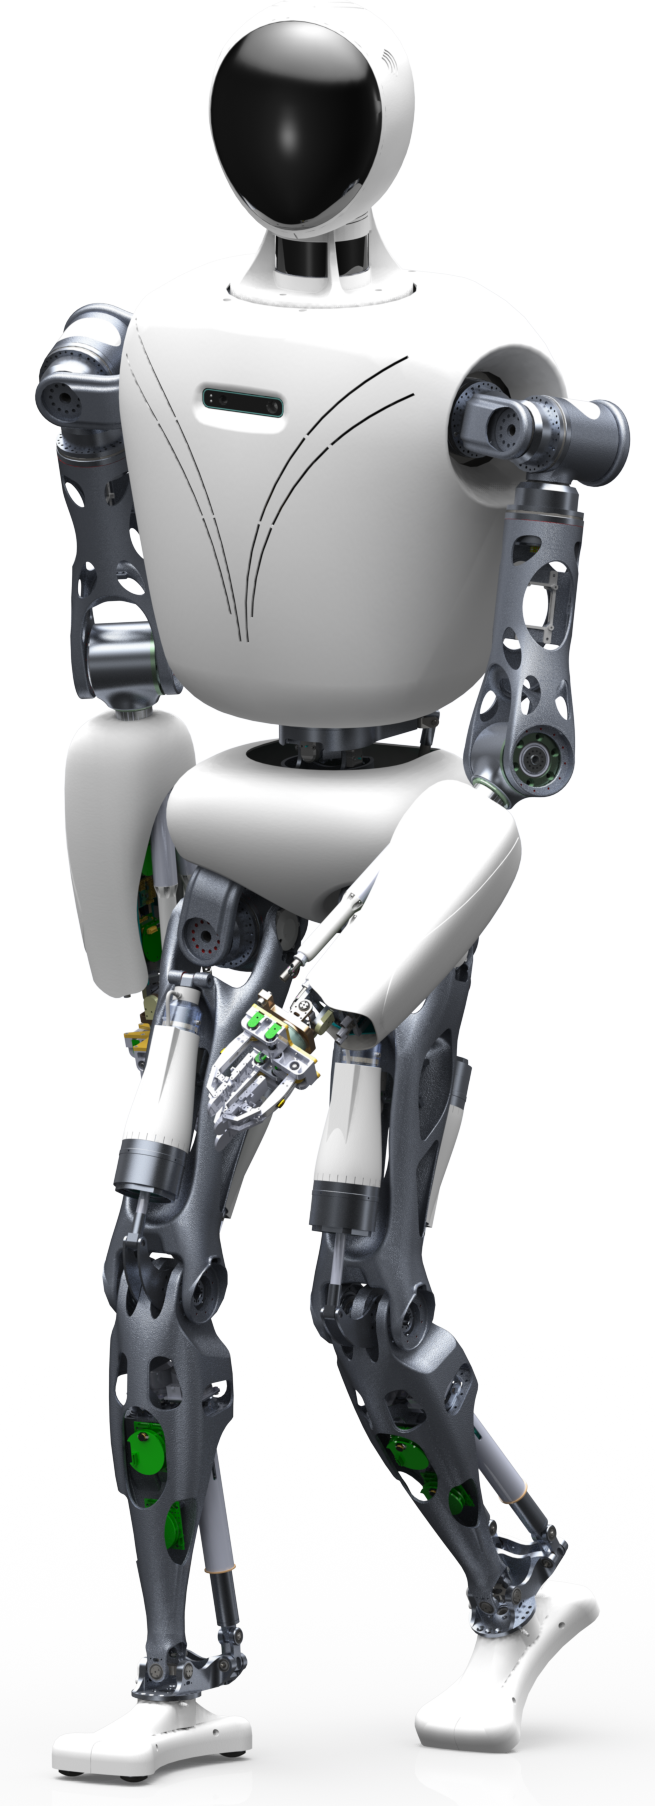
\includegraphics[width=.25\textwidth]{img/rh5_robot.png}
\caption{The recently presented RH5 humanoid is used as experimental platform within this thesis.}
\label{img:rh5_robot}
\end{figure} 

% Add to Appendix: 
% - Gelenkwinkel
% - Gelenkachsen Darstellung
% - URDF (abstract and full)












